\documentclass[11pt,a4paper]{article}
\usepackage[T1]{fontenc}
\usepackage[utf8]{inputenc}
\usepackage[main=italian,provide=*]{babel}
\usepackage{amsmath,amssymb,amsthm}
\usepackage{geometry}
\geometry{margin=2.5cm}
\usepackage{graphicx}
\usepackage{tikz}
\usetikzlibrary{arrows.meta,positioning}
\usepackage{booktabs}
\usepackage{nicematrix}
\usepackage{placeins}
\usepackage{hyperref}
\hypersetup{colorlinks=true,linkcolor=blue,citecolor=blue,urlcolor=blue}

\newtheorem{proposizione}{Proposizione}
\newtheorem{osservazione}{Osservazione}

\title{Dalla composizione dei momenti angolari alla base computazionale:\\
derivazione esplicita degli otto autostati del trimero a catena aperta}
\author{Note di lavoro — Tesi triennale, Samuele Schiavi\\ Relatore: Prof.\ Alessandro Chiesa}
\date{}

\begin{document}
\maketitle

\begin{abstract}
\noindent
Questo documento deriva, passo per passo e senza invocare tabelle di
coefficienti di Clebsch–Gordan come "scatola nera", gli otto autostati
esatti dell'Hamiltoniana del trimero a catena aperta uniforme (blocchi
$A',B',C'$ della decomposizione di Kambe introdotta in
\texttt{teoria\_trimero\_catena\_aperta.pdf}), scritti esplicitamente nella
base computazionale a 3 qubit $|q_1q_2q_3\rangle$. A differenza del caso
dell'anello, qui la coppia usata per la classificazione ($1,3$) non è
adiacente nell'ordine dei qubit del registro ($1,2,3$): il documento tratta
esplicitamente questo riordino, che è l'unica vera differenza tecnica
rispetto al metodo già usato per l'anello
(\texttt{derivazione\_stati\_kambe\_trimero.pdf}).
\end{abstract}

\section{Obiettivo e collocazione}

Nella teoria già sviluppata, l'Hamiltoniana della catena uniforme
\begin{equation}
H = J\,\boldsymbol\sigma_1\cdot\boldsymbol\sigma_2 + J\,\boldsymbol\sigma_2\cdot\boldsymbol\sigma_3 + b\sum_{i=1}^{3}Z_i
\end{equation}
è stata diagonalizzata in forma chiusa sfruttando la conservazione di
$\mathbf S_{13}^2=(\mathbf s_1+\mathbf s_3)^2$, insieme a $\mathbf S^2,S_z$
come sempre. Il risultato erano le energie dei tre multipletti $A'(S_{13}=1,S=3/2)$,
$B'(S_{13}=1,S=1/2)$, $C'(S_{13}=0,S=1/2)$. Qui manca un pezzo: le energie
non dicono chi sono, esplicitamente, i corrispondenti autovettori nella base
$|q_1q_2q_3\rangle$ dei tre qubit — ciò che serve per costruire lo stato
iniziale del circuito VQE.

\textbf{Convenzione qubit.} Come nel resto del progetto, $|0\rangle\equiv{\uparrow}$
(autovalore $Z=+1$), $|1\rangle\equiv{\downarrow}$ (autovalore $Z=-1$).

\textbf{Convenzione di spin vs.\ Pauli.} Per la composizione dei momenti
angolari lavoriamo con $\mathbf s_i=\boldsymbol\sigma_i/2$, per cui
$\mathbf S^2|S,M\rangle=S(S+1)|S,M\rangle$. Gli autovettori di $\mathbf
S^2,S_z$ non dipendono da quale dei due operatori si usa per definirli:
cambia solo la normalizzazione degli autovalori (fattori di conversione già
noti dal resto del progetto), non i vettori. Le energie restano quelle di
\texttt{teoria\_trimero\_catena\_aperta.pdf}; qui interessano solo gli
autovettori.

\section{Il punto delicato: l'ordine di accoppiamento non coincide con l'ordine del registro}
\label{sec:riordino}

Nell'anello, la coppia usata per la classificazione (siti $1,2$) era anche
la coppia \emph{adiacente} nel registro dei qubit $(q_1,q_2,q_3)$: comporre
prima $s_1+s_2$ e poi aggiungere il sito $3$ corrispondeva esattamente
all'ordine naturale del prodotto tensoriale $|q_1q_2\rangle\otimes|q_3\rangle=|q_1q_2q_3\rangle$.

Qui la coppia di classificazione è $(1,3)$, mentre il registro fisico resta
$(q_1,q_2,q_3)$: il sito "spettatore" (site $2$) sta \emph{in mezzo}, non
alla fine. Lavoriamo quindi con un ordine ausiliario "naturale" per la
composizione,
\begin{equation}
|q_1\,q_3\rangle_{13}\otimes|q_2\rangle_2 ,
\end{equation}
e traduciamo alla fine nel registro fisico tramite la corrispondenza
\begin{equation}
|q_1\,q_3\rangle_{13}\otimes|q_2\rangle_2 \;\longleftrightarrow\; |q_1\,q_2\,q_3\rangle_{\text{registro}} .
\label{eq:riordino}
\end{equation}
In pratica: si deriva tutto come se il registro fosse $(1,3,2)$, poi si
scambiano le ultime due cifre di ciascun ket per riportarlo all'ordine
fisico $(1,2,3)$. Questo scambio è l'unica differenza procedurale rispetto
al calcolo già fatto per l'anello — l'algebra di comparazione dei momenti
angolari è identica.

\section{Passo 1 — comporre i due spin della coppia di classificazione (siti 1,3)}

\subsection{Perché si parte da qui}

La simmetria $P_{13}$ rende $\mathbf S_{13}^2=(\mathbf s_1+\mathbf s_3)^2$ una
quantità conservata (dimostrato in \texttt{teoria\_trimero\_catena\_aperta.pdf}).
Conviene quindi costruire una base che sia già autostato di
$\mathbf S_{13}^2$, prima di aggiungere lo spin del sito $2$.

\subsection{Diagonalizzazione esplicita nel settore $M_{13}=0$}

I quattro stati della coppia $(1,3)$ sono $|00\rangle_{13},|01\rangle_{13},|10\rangle_{13},|11\rangle_{13}$
(dove $|q_1q_3\rangle_{13}$ indica $q_1$ del sito $1$, $q_3$ del sito $3$),
autostati di $S_{13,z}=s_{1z}+s_{3z}$ con autovalori $M_{13}=+1,0,0,-1$. Gli
stati $|00\rangle_{13}$ e $|11\rangle_{13}$ sono già non degeneri — autostati
automatici anche di $\mathbf S_{13}^2$. Il settore $M_{13}=0$, generato da
$\{|01\rangle_{13},|10\rangle_{13}\}$, richiede diagonalizzazione esplicita —
\emph{esattamente lo stesso calcolo $2\times2$} già svolto per l'anello (è
pura algebra di due spin $1/2$, non dipende da quali siti fisici siano
coinvolti):
\begin{equation}
\mathbf s_1\cdot\mathbf s_3\;\longrightarrow\;
\begin{pmatrix}-\tfrac14 & \tfrac12\\ \tfrac12 & -\tfrac14\end{pmatrix}
\quad\text{nella base }\{|01\rangle_{13},|10\rangle_{13}\},
\end{equation}
con autovettori $\tfrac1{\sqrt2}(|01\rangle_{13}\pm|10\rangle_{13})$, autovalori
$+\tfrac14$ (simmetrico) e $-\tfrac34$ (antisimmetrico). Tramite
$\mathbf S_{13}^2=\tfrac32\mathbb I+2\,\mathbf s_1\cdot\mathbf s_3$: autovalori
$\tfrac32+2(\tfrac14)=2=1(1{+}1)$ per il simmetrico (tripletto, $S_{13}=1$)
e $\tfrac32+2(-\tfrac34)=0$ per l'antisimmetrico (singoletto, $S_{13}=0$).

\subsection{I quattro stati della coppia di classificazione}

\begin{align}
|S_{13}{=}0\rangle &= \tfrac1{\sqrt2}\big(|01\rangle_{13}-|10\rangle_{13}\big) &&\text{(singoletto)}\label{eq:s13_0}\\
|S_{13}{=}1,M_{13}{=}{+}1\rangle &= |00\rangle_{13} \\
|S_{13}{=}1,M_{13}{=}0\rangle &= \tfrac1{\sqrt2}\big(|01\rangle_{13}+|10\rangle_{13}\big) \\
|S_{13}{=}1,M_{13}{=}{-}1\rangle &= |11\rangle_{13}
\end{align}
Dimensione totale $2\times2=4=1+3$: verificata.

\section{Passo 2 — comporre $S_{13}$ con lo spin del sito 2}

\subsection{Conteggio}

$S_{13}=0$ (dim.\ 1) composto con $j=1/2$ (sito $2$) dà $S=1/2$ soltanto
(dim.\ 2, blocco $C'$). $S_{13}=1$ (dim.\ 3) composto con $j=1/2$ dà $S\in\{1/2,3/2\}$
(dim.\ $2+4=6$, blocchi $B'$ e $A'$). Totale $2+2+4=8$: verificato.

\subsection{Blocco $A'$ ($S=3/2$): costruzione via operatore di abbassamento}

Stato di partenza (banale, un solo modo di avere $M$ massimo):
\begin{equation}
|A',{+}\tfrac32\rangle = |S_{13}{=}1,M_{13}{=}{+}1\rangle\otimes|0\rangle_2 = |00\rangle_{13}\otimes|0\rangle_2 \;\longrightarrow\; |000\rangle
\end{equation}
(qui il riordino della sez.~\ref{sec:riordino} è banale, dato che tutte le
cifre sono $0$).

Operatore di abbassamento totale $S_-=S_{13,-}+s_{2,-}$, con
$S_{13,-}|1,{+}1\rangle_{13}=\sqrt2|1,0\rangle_{13}$,
$S_{13,-}|1,0\rangle_{13}=\sqrt2|1,{-}1\rangle_{13}$, $s_{2,-}|0\rangle_2=|1\rangle_2$
(algebra $su(2)$ standard, identica a quella usata per l'anello):
\begin{align}
S_-|00\rangle_{13}\otimes|0\rangle_2
&= \big(S_{13,-}|00\rangle_{13}\big)\otimes|0\rangle_2 + |00\rangle_{13}\otimes\big(s_{2,-}|0\rangle_2\big)\notag\\
&= \sqrt2\,\tfrac1{\sqrt2}\big(|01\rangle_{13}+|10\rangle_{13}\big)\otimes|0\rangle_2 + |00\rangle_{13}\otimes|1\rangle_2\notag\\
&= \big(|01\rangle_{13}+|10\rangle_{13}\big)\otimes|0\rangle_2 + |00\rangle_{13}\otimes|1\rangle_2 .
\end{align}
Traduciamo ora nel registro fisico tramite \eqref{eq:riordino} ($|q_1q_3\rangle_{13}\otimes|q_2\rangle_2\to|q_1q_2q_3\rangle$):
\begin{align}
|01\rangle_{13}\otimes|0\rangle_2 &\to |q_1{=}0,q_2{=}0,q_3{=}1\rangle = |001\rangle,\\
|10\rangle_{13}\otimes|0\rangle_2 &\to |q_1{=}1,q_2{=}0,q_3{=}0\rangle = |100\rangle,\\
|00\rangle_{13}\otimes|1\rangle_2 &\to |q_1{=}0,q_2{=}1,q_3{=}0\rangle = |010\rangle.
\end{align}
Quindi $S_-|000\rangle = |001\rangle+|100\rangle+|010\rangle$: \emph{lo stesso
insieme di tre stati a singola eccitazione dell'anello}, come deve essere —
è l'insieme di tutti gli stati con un solo qubit a $1$, indipendente da
quale coppia di siti si usi per la classificazione. Dividendo per il
coefficiente $\sqrt{S(S{+}1)-M(M{-}1)}=\sqrt3$ della formula generale:
\begin{equation}
|A',{+}\tfrac12\rangle = \tfrac1{\sqrt3}\big(|001\rangle+|010\rangle+|100\rangle\big).
\label{eq:Ap12}
\end{equation}

\begin{osservazione}
Il blocco $A'$ ($S=3/2$, il multipletto di spin massimo) è la rappresentazione
totalmente simmetrica di $S_3$ (il gruppo delle permutazioni dei tre siti):
è \emph{indipendente dallo schema di accoppiamento}. Per questo
$|A',M\rangle=|A,M\rangle$ per ogni $M$, identici stato per stato a quelli
già derivati per l'anello — non serve rifare il calcolo per $M=-1/2,-3/2$,
ma lo facciamo comunque una volta per completezza e come verifica indipendente.
\end{osservazione}

Applicando $S_-$ una seconda volta (stesso procedimento, sommando i
contributi su ciascuno dei tre termini e traducendo nel registro fisico ad
ogni passo) si ottiene, con coefficiente $\sqrt{\tfrac{15}4-\tfrac12(-\tfrac12)}=2$:
\begin{equation}
|A',{-}\tfrac12\rangle = \tfrac1{\sqrt3}\big(|011\rangle+|101\rangle+|110\rangle\big),
\qquad
|A',{-}\tfrac32\rangle = |111\rangle .
\label{eq:Am12}
\end{equation}
Verificato numericamente (sez.~\ref{sec:verifica}): identici bit per bit ai
corrispondenti stati dell'anello.

\subsection{Blocco $B'$ ($S=1/2$, $S_{13}=1$): stati ortogonali ad $A'$}

\subsubsection{Settore $M={+}1/2$}

I tre stati del registro con un solo qubit a $1$ sono $|100\rangle,|001\rangle,|010\rangle$.
Nella decomposizione pair+spettatore (via \eqref{eq:riordino}):
\begin{align}
|100\rangle &= |10\rangle_{13}\otimes|0\rangle_2, &
|001\rangle &= |01\rangle_{13}\otimes|0\rangle_2, &
|010\rangle &= |00\rangle_{13}\otimes|1\rangle_2 .
\end{align}
Definiamo la base ortonormale del settore $M{=}{+}1/2$
\begin{equation}
e_1 \equiv \tfrac1{\sqrt2}\big(|100\rangle+|001\rangle\big) \quad(\text{da }S_{13}{=}1,M_{13}{=}0\ \otimes\ |0\rangle_2),
\qquad
e_2 \equiv |010\rangle \quad(\text{da }S_{13}{=}1,M_{13}{=}{+}1\ \otimes\ |1\rangle_2).
\end{equation}
Riscriviamo la \eqref{eq:Ap12} in questa base:
\begin{equation}
|A',{+}\tfrac12\rangle = \tfrac1{\sqrt3}\big[(|100\rangle+|001\rangle)+|010\rangle\big]
= \sqrt{\tfrac23}\,e_1 + \sqrt{\tfrac13}\,e_2 .
\end{equation}
(Verifica: $\sqrt{2/3}\cdot\tfrac1{\sqrt2}=\tfrac1{\sqrt3}$, coerente con
l'eq.~\eqref{eq:Ap12}.) Il vettore ortogonale a $(\sqrt{2/3},\sqrt{1/3})$ nel
piano reale $(e_1,e_2)$ è, a meno di fase globale, $(\sqrt{1/3},-\sqrt{2/3})$:
\begin{equation}
|B',{+}\tfrac12\rangle = \sqrt{\tfrac13}\,e_1 - \sqrt{\tfrac23}\,e_2
= \tfrac1{\sqrt6}\big(|100\rangle+|001\rangle\big) - \sqrt{\tfrac23}\,|010\rangle .
\label{eq:Bp12}
\end{equation}
Come nell'anello, questo è automaticamente autostato di $\mathbf S^2$ con
$S=1/2$: essendo $\mathbf S^2$ hermitiano e diagonale a blocchi in ciascun
settore di $M$ fissato, un vettore ortogonale a un autovettore con
autovalore diverso ($S=3/2$) è automaticamente autovettore dell'autovalore
complementare.

\subsubsection{Settore $M={-}1/2$}

Analogamente, i tre stati $|011\rangle,|101\rangle,|110\rangle$ si scompongono come
\begin{align}
|011\rangle &= |01\rangle_{13}\otimes|1\rangle_2, &
|101\rangle &= |11\rangle_{13}\otimes|0\rangle_2, &
|110\rangle &= |10\rangle_{13}\otimes|1\rangle_2 .
\end{align}
Base ortonormale: $f_1\equiv\tfrac1{\sqrt2}(|011\rangle+|110\rangle)$ (da
$S_{13}{=}1,M_{13}{=}0\otimes|1\rangle_2$), $f_2\equiv|101\rangle$ (da
$S_{13}{=}1,M_{13}{=}{-}1\otimes|0\rangle_2$). La \eqref{eq:Am12} diventa
$|A',{-}\tfrac12\rangle=\sqrt{2/3}\,f_1+\sqrt{1/3}\,f_2$, e per ortogonalità:
\begin{equation}
|B',{-}\tfrac12\rangle = \sqrt{\tfrac13}\,f_1-\sqrt{\tfrac23}\,f_2
= \tfrac1{\sqrt6}\big(|011\rangle+|110\rangle\big) - \sqrt{\tfrac23}\,|101\rangle .
\label{eq:Bm12}
\end{equation}

\subsection{Blocco $C'$ ($S_{13}=0$): il caso banale}

Con $S_{13}=0$ non c'è alcuna scelta: comporre spin $0$ con spin $1/2$ dà un
solo multipletto, $S=1/2$, e il sito $2$ resta "spettatore" inerte:
\begin{align}
|C',{+}\tfrac12\rangle &= |S_{13}{=}0\rangle\otimes|0\rangle_2
\;\overset{\eqref{eq:s13_0}}{=}\; \tfrac1{\sqrt2}\big(|01\rangle_{13}-|10\rangle_{13}\big)\otimes|0\rangle_2
\;\longrightarrow\; \tfrac1{\sqrt2}\big(|001\rangle-|100\rangle\big), \label{eq:Cp12}\\
|C',{-}\tfrac12\rangle &= |S_{13}{=}0\rangle\otimes|1\rangle_2
\;\longrightarrow\; \tfrac1{\sqrt2}\big(|011\rangle-|110\rangle\big). \label{eq:Cm12}
\end{align}

\begin{osservazione}
Qui il riordino della sez.~\ref{sec:riordino} produce l'unica vera
differenza visibile rispetto all'anello: nell'anello $|C,+1/2\rangle=\tfrac1{\sqrt2}(|010\rangle-|100\rangle)$
(il sito spettatore, il $3$, compare \emph{a fine} ket); qui il sito
spettatore ($2$) compare \emph{in mezzo} nel bit non coinvolto, e sono i
bit agli \emph{estremi} ($q_1,q_3$) a portare il segno del singoletto:
$|C',+1/2\rangle=\tfrac1{\sqrt2}(|001\rangle-|100\rangle)$. Stessa struttura
fisica (un singoletto su una coppia, spettatore inerte), diversa
"forma" nella stringa di bit — conseguenza diretta di quale coppia è quella
in singoletto.
\end{osservazione}

\FloatBarrier
\begin{figure}[h]
\centering
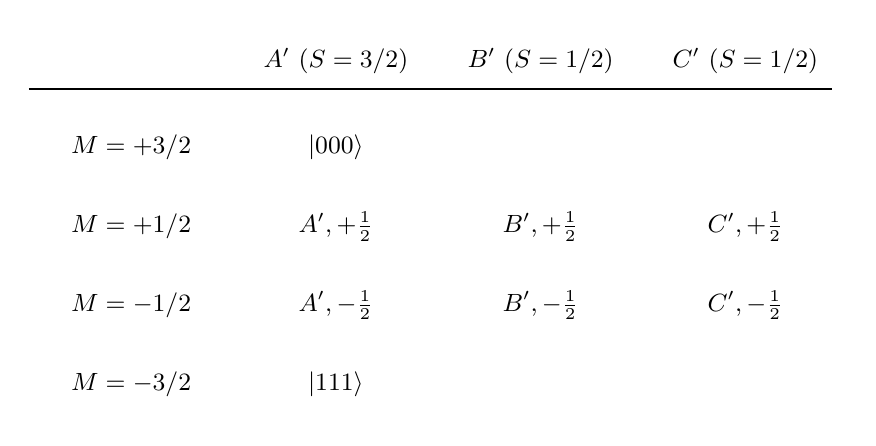
\begin{tikzpicture}[
  every node/.style={font=\small},
  col/.style={minimum width=2.6cm, minimum height=0.85cm, align=center}
]
  % intestazioni di colonna
  \node[col] at (0,0)   {};
  \node[col] at (2.6,0) {$A'$ ($S=3/2$)};
  \node[col] at (5.2,0) {$B'$ ($S=1/2$)};
  \node[col] at (7.8,0) {$C'$ ($S=1/2$)};
  \draw[thick] (-1.3,-0.35) -- (8.9,-0.35);
  % righe M
  \node[col] at (0,-1.1) {$M=+3/2$};
  \node[col] at (2.6,-1.1) {$|000\rangle$};

  \node[col] at (0,-2.1) {$M=+1/2$};
  \node[col] at (2.6,-2.1) {$A',{+}\tfrac12$};
  \node[col] at (5.2,-2.1) {$B',{+}\tfrac12$};
  \node[col] at (7.8,-2.1) {$C',{+}\tfrac12$};

  \node[col] at (0,-3.1) {$M=-1/2$};
  \node[col] at (2.6,-3.1) {$A',{-}\tfrac12$};
  \node[col] at (5.2,-3.1) {$B',{-}\tfrac12$};
  \node[col] at (7.8,-3.1) {$C',{-}\tfrac12$};

  \node[col] at (0,-4.1) {$M=-3/2$};
  \node[col] at (2.6,-4.1) {$|111\rangle$};
\end{tikzpicture}
\caption{Diagramma dei livelli in $M$ per i tre blocchi. $A'$ occupa i
quattro valori $M=\pm3/2,\pm1/2$; $B'$ e $C'$, entrambi $S=1/2$, occupano
solo $M=\pm1/2$ ma sono stati fisicamente distinti (diverso $S_{13}$,
diversa energia — vedi teoria). Struttura identica a quella dell'anello,
solo l'etichetta $S_{12}\to S_{13}$ cambia.}
\end{figure}
\FloatBarrier

\section{Riepilogo e verifica numerica}
\label{sec:verifica}

\begin{table}[h]
\centering
\begin{tabular}{@{}llll@{}}
\toprule
Blocco & $S$ & $M$ & Stato esplicito (registro $|q_1q_2q_3\rangle$)\\
\midrule
$A'$ & $3/2$ & $+3/2$ & $|000\rangle$\\
$A'$ & $3/2$ & $+1/2$ & $\tfrac1{\sqrt3}(|001\rangle+|010\rangle+|100\rangle)$\\
$A'$ & $3/2$ & $-1/2$ & $\tfrac1{\sqrt3}(|011\rangle+|101\rangle+|110\rangle)$\\
$A'$ & $3/2$ & $-3/2$ & $|111\rangle$\\
$B'$ & $1/2$ & $+1/2$ & $\tfrac1{\sqrt6}(|100\rangle+|001\rangle) - \sqrt{2/3}\,|010\rangle$\\
$B'$ & $1/2$ & $-1/2$ & $\tfrac1{\sqrt6}(|011\rangle+|110\rangle) - \sqrt{2/3}\,|101\rangle$\\
$C'$ & $1/2$ & $+1/2$ & $\tfrac1{\sqrt2}(|001\rangle-|100\rangle)$\\
$C'$ & $1/2$ & $-1/2$ & $\tfrac1{\sqrt2}(|011\rangle-|110\rangle)$\\
\bottomrule
\end{tabular}
\caption{Gli otto stati derivati, in base computazionale $|q_1q_2q_3\rangle$.}
\label{tab:stati}
\end{table}

\textbf{Confronto diretto con l'anello.} $A'\equiv A$ stato per stato (già
atteso, sez.~4.2). $C'$ ha la stessa struttura di $C$ ma con il singoletto
sui bit estremi invece che sui bit $2,3$. $B'$ ha la stessa struttura a tre
termini di $B$, ma con i pesi $2{:}1{:}1$ ridistribuiti sui bit
corrispondenti alla nuova coppia di classificazione.

\textbf{Verifica indipendente (autotest numerico).} Gli otto vettori sono
stati verificati con NumPy contro $H$ dell'eq.~(1) in convenzione di Pauli
diretta (stessa funzione \texttt{H\_chain} di \texttt{verifica\_catena\_preliminare.py}),
al punto $(J,b)=(1.3,-0.7)$ scelto casualmente (nessuna simmetria
accidentale che potrebbe mascherare un errore):

\begin{table}[h]
\centering
\begin{tabular}{@{}lccc@{}}
\toprule
Stato & $\|\psi\|^2$ & $E_{\text{num}}=\langle\psi|H|\psi\rangle$ & $E_{\text{teor}}=E(S_{13},S)+2bM$\\
\midrule
$A',{+}3/2$ & $1.000000000$ & $0.50000$ & $0.50000$\\
$A',{+}1/2$ & $1.000000000$ & $1.90000$ & $1.90000$\\
$A',{-}1/2$ & $1.000000000$ & $3.30000$ & $3.30000$\\
$A',{-}3/2$ & $1.000000000$ & $4.70000$ & $4.70000$\\
$B',{+}1/2$ & $1.000000000$ & $-5.90000$ & $-5.90000$\\
$B',{-}1/2$ & $1.000000000$ & $-4.50000$ & $-4.50000$\\
$C',{+}1/2$ & $1.000000000$ & $-0.70000$ & $-0.70000$\\
$C',{-}1/2$ & $1.000000000$ & $0.70000$ & $0.70000$\\
\bottomrule
\end{tabular}
\end{table}

Errore massimo su energia e norma $<10^{-15}$; massimo elemento fuori
diagonale della matrice di Gram (ortogonalità reciproca) $6.7\times10^{-17}$.
Inoltre, per ciascuno stato è stato verificato $\|H|\psi\rangle-E_{\text{teor}}|\psi\rangle\|\sim10^{-16}$:
sono autovettori esatti, non solo a valore d'aspettazione corretto —
massimo residuo $9.9\times10^{-16}$ su tutti e otto gli stati.

\section{Struttura degli stati: cosa significa per la preparazione su circuito}

\begin{table}[h]
\centering
\begin{tabular}{@{}lll@{}}
\toprule
Stato & Struttura & Preparazione\\
\midrule
$C',\pm1/2$ & prodotto singoletto$_{13}\otimes|\cdot\rangle_2$ & non banale: singoletto su qubit \emph{non adiacenti}\\
$A',\pm3/2$ & stato prodotto puro & banale: solo porte $X$\\
$A',\pm1/2$ & sovrapposizione a 3 termini, pesi uguali & stato di tipo $W$, stessa preparazione dell'anello\\
$B',\pm1/2$ & sovrapposizione a 3 termini, pesi $2{:}1{:}1$ & stessa famiglia di $A_{1/2}$, pesi/segni diversi\\
\bottomrule
\end{tabular}
\caption{Complessità di preparazione dei diversi stati.}
\end{table}

\begin{osservazione}[Differenza pratica rilevante rispetto all'anello]
Nell'anello, $|C,\pm1/2\rangle$ era il singoletto sui qubit \emph{adiacenti}
$1,2$ — preparabile con la stessa sequenza a due qubit del dimero (X, H,
CNOT, X), col terzo qubit spettatore. Qui $|C',\pm1/2\rangle$ è il
singoletto sui qubit $1,3$, che nel registro fisico \emph{non sono
adiacenti} (il qubit $2$ sta in mezzo): la sequenza standard
Hadamard+CNOT prepara un singoletto fra qubit adiacenti sul circuito, quindi
servirà o un SWAP (costo aggiuntivo) o una CNOT non locale fra i qubit $1$
e $3$ (dipende dalla connettività del backend). Questo è un punto tecnico
da tenere presente quando si passa all'implementazione del circuito VQE
(Fase 4): il candidato più semplice per lo stato iniziale non è più "gratis"
come lo era per l'anello.
\end{osservazione}

\section{Collegamento con il seguito}

Con gli otto stati espliciti disponibili, i candidati come stato iniziale
del PMA per il VQE a 3 qubit sulla catena sono già identificati (Tabella
\ref{tab:stati}). Dato che, dalla sez.~6 di \texttt{teoria\_trimero\_catena\_aperta.pdf},
per $J>0$ (regime antiferromagnetico) il fondamentale a campo debole è nel
blocco $B'$ — non $C'$ come nell'anello nel punto di lavoro consueto — lo
stato iniziale naturale per il primo test end-to-end su questa topologia
sarà $|B',-1/2\rangle$, che richiede comunque una preparazione non banale
(Tabella 3): non c'è, per questa topologia, un analogo "gratuito" del
singoletto del dimero come punto di partenza a campo debole.

\appendix
\section{Riepilogo delle formule}

\begin{align*}
|S_{13}{=}0\rangle &= \tfrac1{\sqrt2}(|01\rangle_{13}-|10\rangle_{13}) &
|S_{13}{=}1,0\rangle &= \tfrac1{\sqrt2}(|01\rangle_{13}+|10\rangle_{13})\\[4pt]
|A',{+}\tfrac32\rangle &= |000\rangle &
|A',{-}\tfrac32\rangle &= |111\rangle\\
|A',{+}\tfrac12\rangle &= \tfrac1{\sqrt3}\big(|001\rangle+|010\rangle+|100\rangle\big) &
|A',{-}\tfrac12\rangle &= \tfrac1{\sqrt3}\big(|011\rangle+|101\rangle+|110\rangle\big)\\
|B',{+}\tfrac12\rangle &= \tfrac1{\sqrt6}(|100\rangle+|001\rangle) - \sqrt{\tfrac23}|010\rangle &
|B',{-}\tfrac12\rangle &= \tfrac1{\sqrt6}(|011\rangle+|110\rangle) - \sqrt{\tfrac23}|101\rangle\\
|C',{+}\tfrac12\rangle &= \tfrac1{\sqrt2}(|001\rangle-|100\rangle) &
|C',{-}\tfrac12\rangle &= \tfrac1{\sqrt2}(|011\rangle-|110\rangle)
\end{align*}
Operatore di abbassamento usato: $S_-|S,M\rangle=\sqrt{S(S{+}1)-M(M{-}1)}\,|S,M{-}1\rangle$
(risultato standard dell'algebra $su(2)$, non ridimostrato).

\end{document}
